\section{LDLM: Lock Manager}

The basic design idea of Lustre Lock Manager comes from VAX DLM. There
are some fundamental concepts we need to explain before we can dive into
the code and understand how it works.

\subsection{Namespace}

The first concept we will cover is the \textit{namespace}. Whenever you request a
lock, you are asking a lock for a certain resource in a namespace, and there is
one namespace defined per Lustre service.  To put this in a practical context,
say your Lustre system is composed of ten OSTs, then from LDLM point of view,
there are ten namespaces.  Furthermore, MDS and MGS each have their own
namespaces here. A namespace in Lustre is defined by struct
\url{ldlm_namespace}. It has a reasonable amount of comments for the fields in the
source code, so here we just focus on a few of the less-obvious ones.

\begin{figure}[htb]
\centering
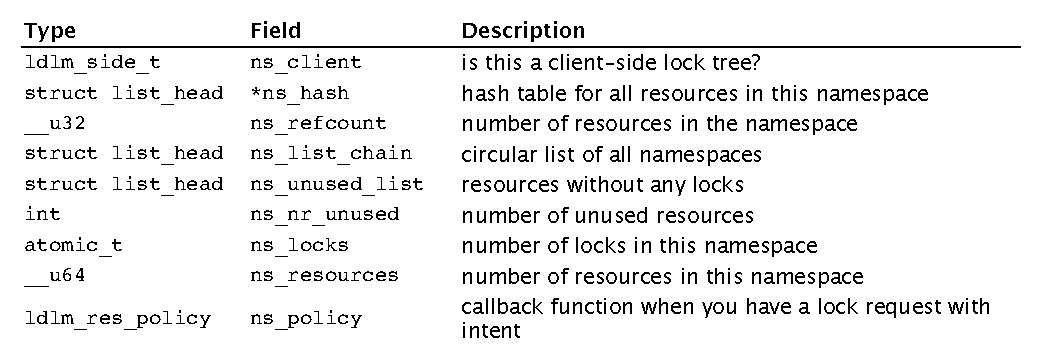
\includegraphics[width=5in]{img/lustre_ns}
\caption{The fields of \textit{ldlm\_namespace} data structure.}
\label{fig:ns}
\end{figure}

Some additional notes on \url{ns_client}: Each client only needs access to
some portions of a namespace, but not all of them. So each client carries a
so-called \textit{shadow namespace}.  \url{ns_client} is a flag that says this
namespace is for client only and is not complete (see Figure~\ref{fig:shadow} for an
illustration). \url{ns_hash} is a hash table for all resources in this
namespace. Notice that this is a pointer to the linked list, not just the
linked list itself.

\begin{figure}[htb]
\centering
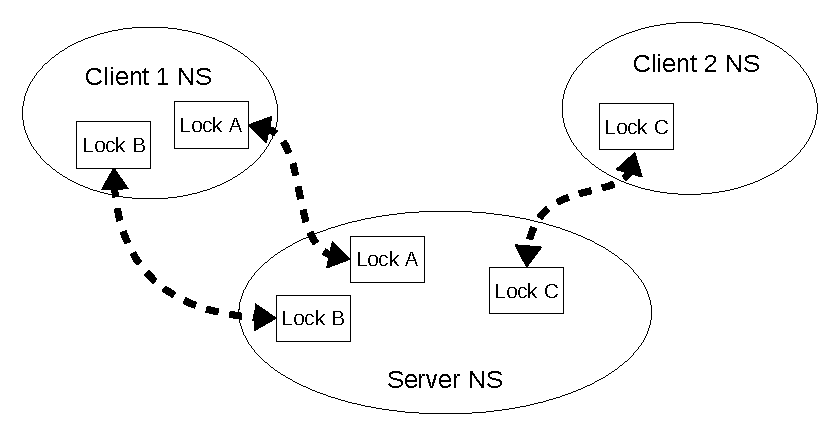
\includegraphics[width=3.5in]{img/lustre_nsclient}
\caption{Shadow namespaces on clients.}
\label{fig:shadow}
\end{figure}

\subsection{Resource}

A lock is for protecting resources. In Lustre, the most common type of
resources are files. A \textbf{local lock} refers to a lock that is private,
known only to the local entity. Correspondingly, a \textbf{global lock} is
visible to the others.  Note that ``global'' in this case may be a misnomer
-- it doesn't mean the lock is actually broadcast and known by all parties.
In Lustre, it means you have a client copy of the lock, but server also got a
copy through client request.\footnote{The lock on the server may be called 
the master lock.}

A resource is defined in struct \url{ldml_resource}. Some highlights of the
struct are discussed below.

\begin{description}

\item[\url{struct ldlm_namespace *lr_namespace}]

Points back to the namespace this resource belongs to. If the resource
is a object id (oid), then its namespace is the associated OST. If it is fid,
then its namespace is defined by the MDS.

\item[\url{struct list_head lr_granted, lr_converting, lr_waiting}]

There are three lists defined here to categorize different locks and their
states requested on this resource. \textit{Granted list} is for all locks that
have been granted use on this resource. \textit{Waiting list} is for locks
requesting the resource, but must wait due to a conflict.  \textit{Converting
list} is for locks changing mode. 

\item[\url{struct ldlm_res_id lr_name}] 

The name of the resource is defined in a struct, which is a 4$\times$64 bits long
identifier.  All types of resources, either fid or oid, will be converted to
this format as their generic resource name.

\end{description}


\subsection{Lock Type and Mode}

A lock has both a type and a mode. We discuss the mode first. There are
six lock modes along with a compatibility matrix to indicate if two
locks are compatible. The six modes are given below.

\begin{itemize}

\item \url{EX} \textbf{Exclusive mode} Before a new file is created, MDS
requests \url{EX} lock on the parent.

\item \url{PW}  \textbf{Protective Write (normal write) mode} When a client
requests a  write lock from an OST, a lock with PW mode will be issued.

\item \url{PR}  \textbf{Protective Read (normal read) mode} When a client
requests a read from an OST, a lock with \url{PR} mode will be issued. Also, if
the client opens a file for execution, it is granted a lock with \url{PR} mode.

\item \url{CW}  \textbf{Concurrent Write mode} The type of lock that the MDS
grants if a client requests a write lock during a file open operation.

\item \url{CR}  \textbf{Concurrent Read mode} When a client performs a path
lookup, MDS grants \url{inodebit} lock with the \url{CR} mode on the
intermediate path component.

\item \url{NL}  \textbf{Null mode}.

\end{itemize}

The corresponding matrix is given in Figure \ref{fig:matrix}.

\begin{figure}[htb]
\centering
\begin{Verbatim}
                                 NL  CR  CW  PR  PW  EX
                             -----------------------------
                            NL    1   1   1   1   1   1
                            -----------------------------
                            CR    1   1   1   1   1   0 
                            -----------------------------
                            CW    1   1   1   0   0   0  
                            -----------------------------
                            PR    1   1   0   1   0   0
                            -----------------------------
                            PW    1   1   0   0   0   0 
                            -----------------------------
                            EX    1   0   0   0   0   0 
                            -----------------------------
\end{Verbatim}
\caption{Lock compatibility matrix.}
\label{fig:matrix}
\end{figure}

In Lustre, four types of locks are defined, and it is up to the client to decide
what type of lock it requests.  The component that requests a lock from the
lock manager is the client, and it can be Lustre Lite, OSC or MDC. These four
types of locks are given below. 

\begin{description}

\item[\textit{extent lock}] for protecting OST data, defined by struct
\url{ldlm_extent}.

\item[\textit{flock}] for supporting a user space request on flock, defined by
struct \url{ldlm_flock}.

\item[\textit{inode bit lock}] for protecting metadata attributes, defined by
struct \url{ldlm_inodebits}.

\item[\textit{plain lock}] defined, but not in use and can be ignored.

\end{description}

\subsection{Callbacks}

Another concept associated with the lock request is the \textit{callback
function}. When a lock is created, a client can supply three type of callbacks:

\begin{description}

\item[\textit{blocking callback}] There are two conditions where this callback
will be invoked. First, if a client requests a lock conflicting with this one
(even if the request comes from the same client), then this callback is invoked,
so that if this client plays ``nice'' and has no use for this lock anymore, it
can release the lock and let the other party have it. The second case is when a
lock is revoked (after all references went away and the lock was cancelled).

\item[\textit{completion callback}] There are also two cases in which this callback will
be invoked: first, if the lock requested is granted; second, if the lock is
converted, for example, to a different mode.

\item[\textit{glimpse callback}] This callback is used to provide certain
information about underlying properties without actually releasing the lock.
For example, an OST can provide such a callback to provide information on file
size since only the OSTs know exactly the size of a file object. This callback
is then associated with the extent lock on the file object and is invoked by
the server upon receiving the client request.

\end{description}


\subsection{Intent}

An intent is a piece of data supplied with a lock enqueue indicating special
processing is needed during lock enqueue, and the data themselves are the parameters
for that processing. Namespaces can have different \textit{intent handlers}
defined for such processing.

The intent feature allows the caller of~\url{namei} and lookup to pass some information
about what they want to accomplish in the end. The net effect of this is a
reduced number of RPC requests when interacting with the MDS.

A intent is defined as follows (\url{inode.h}):

\begin{Verbatim}
struct intent {
    unsigned    int_opmask;
    void        * int_arg1;
    void        * int_arg2;
};
\end{Verbatim}

Six intention operations are defined (encoded in \url{int_opmask}). These
are get attributes, set attributes, insert or delete, open, create, and
read links.

\subsection{Lock Manager}

Now let's provide a general description of how the locking algorithm
(implemented by the lock manager) works in Lustre.  The entry call to Lustre
Distributed Lock Manager (LDLM) changes with different Lustre versions; we take
1.6 branch code as our reference. There are two major types of requests an
LDLM can service: first, when a lock is requested, and second, when a lock is
cancelled. We describe the two cases separately.

\subsubsection{Requesting a Lock}
\label{sec:requestlock}

\begin{enumerate}

\item A locking service client, whether it is a Lustre client, MDS, or OST,
usually starts with a call to \url{ldlm_cli_enqueue()}. This function first
examines if the lock requested belongs to the local namespace by checking the
flag \url{ns_client} in the namespace struct.  Remember that each LDLM instance
defines its own namespace.  If it is local, meaning that we don't have to send
RPC to communicate, we skip to step \ref{lm:local}; otherwise, we continue
processing the lock remotely.

\item If the lock request is for a non-local namespace, we need to send
\textit{lock enqueue RPC} to LDLM running on the server; this is done inside
the \url{ldlm_cli_enqueue()}. On the server side, \url{ldlm_handle_enqueue()}
unpacks the lock request first, then creates a lock (\url{ldlm_lock_create()}).
This lock is just an initial one with some fields filled in from the original
lock request; it has not been granted yet. You can determine if a lock is
granted or not by checking:

    \begin{Verbatim}
    if (lock->req_mode == lock->granted_mode) {   /* granted */
        ...
    }
    \end{Verbatim}

Now we move to the next step to check if the lock can be granted and what lock
should be granted.

\item \url{ldlm_lock_enqueue()} is the core step for granting the lock. It
checks if the lock intent is set. If no intent is set, then it checks for the
lock type and invokes the policy function defined for this lock type. The
policy function will determine if the request lock can be granted or not. 

If the lock intent is set, go to step \ref{lm:intent}.

\item For the resource for which the lock is being requested, two conditions
need to be checked as given below.
  
  \begin{itemize}
  \item Are there any conflicts with those granted locks?
  \item Are there any conflicts with those waiting locks?
  \end{itemize}

If the answer to both questions is no, then no conflict is found, and the lock can be granted.
Call \textit{completion AST}\footnote{AST is the acronym for Asynchronous System
Trap from VMS lock design. Here, we consider it to be synonymous with a
callback.}, return the granted lock, and we are done.  Otherwise, continue.

\item For each conflicting lock, we need to call \textit{blocking AST}.
Blocking AST checks if the lock is held at the server, then just sets a flag. If
the lock is held at the client, then a \textit{blocking RPC} request must be
sent. Either way, after all these are done, put this new lock request on the
waiting list, then return the lock with status as being blocked.

A more detailed policy function implementation is provided later.

\item \label{lm:intent} If the lock intent is set, then all that needs to be done is to
invoke the intent handler. The key point is that LDLM does not interpret intents. The
parties communicating with each other with intent do that; for example, MDS needs to
register its intent handler, and OST needs to register its intent handler. In general,
intent handler is registered per namespace by calling
\url{ldlm_register_intent()}. It is the LDLM's responsibility to invoke them.
The intent handler will determine if the lock can be granted or not. LDLM just
returns the result of their verdict.

\item \label{lm:local} For a local lock request, it goes to a different branch
at \url{ldlm_cli_enqueue_local()}, except that in this case it doesn't need to
send an RPC anymore. It will need to go through the two phases described above:
creating a lock first, then calling \url{ldlm_lock_enqueue()} to check if this
can be granted. If either lock is granted or if there are any errors, it
returns immediately with the lock marked correspondingly. Otherwise, lock request
is being blocked, and it needs to wait for it.

Please note that a server (e.g., MDS or OST) can initiate a lock request by
directly calling \url{ldlm_cli_enqueue_local()} since they know the lock must
be held by the local LDLM server. 

\end{enumerate}

\subsubsection{Canceling a Lock}

A lock is usually released involuntarily, and the owner will hold it as long as
possible until: someone is asking for a conflicting lock, LDLM sends out
a blocking AST, and the block AST handler invoked on the LDLM client side. Now we enter
the canceling process.  There are three counters in the lock that are related
to the cancelling process. These can be listed as (1) counts of active
readers, (2) counts of active writers, and (3) counts of users.

\begin{enumerate}

\item The entry point for cancelling a lock is \url{ldlm_cli_cancel()}. This
function first checks if the sum of active readers and writers is zero. If not,
it means another process on the same client is using the lock so, we do
nothing.  Eventually, the other client(s) will release the lock and follow the
same code path and reach this checkpoint, then it will move to the next
step.

\item Now when the sum of readers and writes count reaches zero, we call blocking
AST with a flag set indicating this lock is being revoked. 

\item Check if this lock is in the local namespace. If it is not, send
\textit{cancel RPC} to client (Lustre client). If so, the server side calls
\url{ldlm_handle_cancel()} to cancel the lock.

A cancel operation essentially involves steps that take this lock of all the
lists it is currently on, such as granted list, waiting list, etc. Later,
\url{obd_cancel()} will be called not to cancel the lock, but just to release
the references on reader and writer counts.

\item Now that the lock has been cancelled, server can reprocess all waiting locks
on the resource. It essentially goes through the same logic to determine if
their lock requests can be granted.

\item If a waiting lock request can be granted, move it to the granted lock
list, then invoke the \textit{completion AST}.

\end{enumerate}

\subsubsection{Policy Function}

As we discuss in the section on requesting a lock (\ref{sec:requestlock}),
policy function is being called to determine if the requested lock is in
conflict with existing requests, based on the lock type. We have four lock
types, and these are \textit{inodebits}, \textit{extent}, \textit{flock}, and
\textit{plain}. Therefore, we need four policy functions. They all follow a
similar overall flow, with some minor changes.  In this section, we give
an overall description on the overall flow.

\begin{enumerate}

\item There are two given parameters and these are lock request and a flag of
\url{first_enq}. This flag means to signal if this is first time we do an
enqueue request. If this is the first time, the waiting list needs to be processed
and send blocking ASTs when necessary. If this is not the first time, then we
already sent out blocking AST before, so there is no need to do it again.

Another important thing about \url{first_enq} parameter is that when it is not set
(which means we are reprocessing a lock already in the waiting list),
we stop processing the waiting list after we find our own earlier entry in the
list. Since the rest of the locks were enqueued at a later point in time, those
can be ignored safely.


\item \label{lm:helper} The policy function calls on a helper function for
real work, passing in as parameters both lock list, enqueue flag, as well as a
RPC list, either \url{NULL} or a empty list. The first time, the helper
function is called with a granted lock list. For each lock in the list, it
performs the following conflict detection.\footnote{An implementation can
choose to implement its own policy function and conflict detection, not
necessarily follow exactly as we presented here.}

  \begin{enumerate}

  \item It always starts with mode checking. If two locks are compatible (refer
  	to the previous section for the compatibility matrix), then no more checking is
  	needed, and a lock can be granted. We continue only if locks are incompatible and the lock
  	type is not \textbf{plain} since plain lock is not actually in use.

  \item For the \textbf{extent} lock type, if the interval or range does not 
  	intersect, then there is no conflict. However, within the boundary of a stripe 
	size, LDLM always tries to grant the largest extent possible to reduce the 
	possibility of further requests in case the client asks for more locks.

  \item For the \textbf{inodebits} lock type, if the bits requested (Lustre has a
	64-bit lock space, but only 3 are being used) intersect, then there are
	conflicts.  \footnote{It groups locks based on the bits (more precisely, it is
	based on the integers formed by the 3-bit value since only 3-bits are in use),
	so you only need to check one member in each group to make a decision, as a
	performance optimization.}

  \end{enumerate}

If the RPC list is \url{NULL}, we stop and return right after the first
conflict is detected, since by passing \url{NULL}, we obtained all the
information that the caller requires. 

If the RPC list is not \url{NULL}, we need to continue for each remaining locks
and add the conflicting lock into the RPC list.


\item If no conflicts are found, then the lock is granted. Otherwise, for each
conflict lock in the RPC list, we invoke blocking AST.


\item If first enqueue flag is set, then we go back to step \ref{lm:helper},
but this time, we invoke the helper function with the lock list set as waiting list
instead of granted list.


\end{enumerate}


\subsection{Use Cases}

In this section, we use examples to give high level overview on
processing lock requests.

\subsubsection*{MDS: One Client Read}

Let's assume client $C_1$ wants to open the file \url{/d1/d2/foo.txt} to read.
During the VFS path lookup, Lustre specific lookup routine will be invoked (see the
Lustre Lite section for details on this). The first RPC request is lock enqueue
with lookup intent. This is sent to MDS for lock on \url{d1}. The second RPC
request is also lock enqueue with lookup intent and is sent to MDS asking
inodebits lock for \url{d2}. The lock returned is an inodebits lock, and its
resources would be represented by the fid of \url{d1} and \url{d2}.

The subtle point to note is, when we request a lock, we generally need a
resource id for the lock we are requesting. However in this case, since we
don't know the resource id for \url{d1}, we actually request a lock on its
parent \url{/}, not on the \url{d1} itself. In the intent, we specify it as a
lookup intent and the name of the lookup is \url{d1}. Then, when the lock is
returned, the lock is for \url{d1}. This lock is (or can be) different from
what the client requested, and the client notices this difference and replaces
the old lock requested with the new one returned.

The third RPC request is a lock\_enqueue with open intent, but it is not asking for
lock on \url{foo.txt}.\footnote{Lustre Lite always decides no need for a lock
unless it is from NFS.} That is, you can open and read a file without a lock
from MDS since the content is provided by OST.  Requesting locks from an OST is
a different matter and is discussed later.

In other words, what happens at open is that we send a lock\_request, which
means we \textit{do} ask for a lock from LDLM server.  But, in the intent data itself, we
might (or not) set a special flag if we are actually interested in receiving
the lock back. And the intent handler then decides (based on this flag),
whether or not to return the lock.


If \url{foo.txt} exists previously, then its  fid, inode content (as in owner,
group, mode, ctime, atime, mtime, nlink, etc.) and striping information are
returned.

If client $C_1$ opens the file with the \url{O_CREAT} flag and the file doesn't
exist, the third RPC request will be sent with open and create intent, but
still there will be no lock requests. Now on the MDS side, to create a file
\url{foo.txt} under \url{d2}, MDS will request through LDLM for another
\url{EX} lock on the parent directory. Note that this is a conflicting lock
request with the previous \url{CR} lock on \url{d2}. Under normal
circumstances, a fourth RPC request (blocking AST) will go to client $C_1$ or
anyone else who may have the conflicting locks, informing the client that
someone is requesting a conflicting lock and requesting a lock cancellation.
MDS waits until it gets a cancel RPC from client. Only then does the MDS get the
\url{EX} lock it was asking for earlier and can proceed.\footnote{In the current
code, client gets smart. When it sees that it will create a new file, it cancels
the lock on \url{d2} itself by embedding the cancel operation on the third RPC
request. This saves two RPCs, one blocking AST from MDS to client and one
cancel RPC from client to MDS.}
 
If client $C_1$ opens the file with \url{LOV_DELAY} flag, MDS creates the file
as usual, but there is no striping and no objects are allocated. User will
issue an \url{ioctl} call and set the stripe information, then the MDS will
fill in the EA structure.

\subsubsection*{MDS: Two Clients}

If $C_1$ wants to create a file \url{foo.txt} under the directory \url{/d1/d2},
then no locks are required on \url{foo.txt}, but it will request a lock on
\url{d2} with the intent of instructing MDS to ``open and create" the file
\url{foo.txt} and possibly to return a lock on that file.

It acquires a \url{CW} lock intentionally on \url{foo.txt}.  Now $C_2$ comes in
and wants to create a new directory \url{d3} under \url{/d1/d2}. At this point
nothing will change as far as the \url{CW} lock is concerned.

\subsubsection*{OST: Two Clients Read and Write}

After the MDS fills in the EA structure, the client has the file handle and
stripe information. The client can now talk to OSTs. Let's assume we have four OSTs
and two clients. Client $C_1$ reads file $A$ and the second client $C_2$
writes to file $A$. We further assume that $C_1$ wants to read data objects,
$A_1$, $A_2$, $A_3$, and $A_4$.

First, client $C_1$ sends lock enqueue requests to OSTs 1 through 4 in
parallel, asking for read lock with intent flag set. What it means is, if any
of the objects client $C_1$ is asking has a blocking request, don't try to get
the lock, just return back the information (file size, modification time, etc.)
described by a data structure called \url{lvb} (Lustre Value Block) (the lock
request is a glimpse because it has intent flag set). 

If there are no conflicts, the client will be granted read locks on the
entire file objects, with lock mode as \url{PR}. Now the client has four read
locks on four OST file objects. Let's further assume that the client only wants to
read $A_1$. Since it has the lock, it can now go ahead and read it.

Assume $C_2$ is writing to OST3. Instead of returning a \url{PR} lock, OST3
will contact $C_2$ and ask for the \url{lvb} information. It then would return
this format back to $C_1$: ``I am not issuing you the lock on $A_3$, but here
is the state of that object''.

This was done just to determine the file size, and we need to know the file size,
for example, if we are trying to read beyond the file size.  If the content of
read falls into the object you already hold a \url{PR} lock on, then no further
RPCs for that lock are needed.

Now if the content the client needs to read is on $A_3$, then it has no choice
but to send a read lock request (without intent this time) to OST3.  Within the
request itself, the client should also make clear to what \textit{extent} it is
requesting the lock. If the extent it is requesting is not conflicting
(intersecting reads) with the \url{PW} write lock $C_2$ is holding, then the
read lock request will be immediately granted.

If a conflict exists, then OST3 will reply to $C_1$ that the lock request is
not granted and at the same time, it will send a blocking request to $C_2$.
There are two cases to consider from the perspective of $C_2$:

\begin{enumerate}

    \item If the \url{write()} system call is done, meaning that all data has
    been written to some buffer (maybe not to disk yet), then the buffers will
    have the dirty flag set. In that case, the client flushes all dirty buffers, probably
    through one or more bulk writes. Then it releases the lock (lock
    reference count is now zero) by sending a cancel RPC to OST3.

    \item If the \url{write()} is still in progress, then the system call
    hasn't returned yet. At this point, the lock reference count is non-zero and
    the blocking AST won't reach the lock logic.
    Only after the write system call finishes (it actually means at
    least two things here, one, the data is all in cache and two, the lock
    reference count is decreased to zero), then it can go to the step explained above.

\end{enumerate}

After OST3 gets the cancel request from $C_2$, it will send a completion
AST to client $C_1$, telling that now its lock request is granted.

We don't explain a case where both clients do read because it is trivial, as  
both of them can get \url{PR} locks, even with their extent intersecting.

If one client doesn't play nice and doesn't cooperate in releasing its lock,
then a timer is started the moment it was sent a blocking AST. If the client
doesn't release the lock and there is no ongoing I/O under that lock for the
duration of the timeout, then the client is evicted. However, if there is
ongoing I/O, then on every I/O RPC the timeout is prolonged.

\begin{comment}
the OST3 checks the last bulk write and starts the
obd timeout, when it expires without receiving another bulk write, the
client will be evicted.
\end{comment}

\begin{comment}

int flock(int fd, int operation)

- it is advisory

   - it apply to entire file

- three operations: LOCK_SH (shared), LOCK_EX (exclusive), LOCK_UN
(remove existing lock by this process)

- locks created by flock() are associated with a open file. multiple
process may point to the same lock, say when dup() is called.

- a lock is released when LOCK_UN operation is done on any of
these duplicate descriptors, or when all such descriptors have been
closed.

- A process may only hold one TYPE of lock (shared or exclusive) on a
file. Subsequent flock() call on an already locked file will convert an
existing lock to the new lock mode.



One of the first three will be part of so called policy data, defined as a
union:

    typedef union {
        struct ldlm_extent      l_extent;
        struct ldlm_flock       l_flock;
        struct ldlm_inodebits   l_inodebits;
    } ldlm_policy_data_t;




    struct list_head    l_lru;
    struct list_head    l_res_link;
    struct list_head    l_extents_list;
    struct list_head    l_cache_locks_list;
    struct list_head    l_pending_chain;
    struct hlist_node   l_exp_hash;
    struct list_head    l_bl_ast;
    struct list_head    l_bp_ast;
    struct list_head    l_sl_mode;
    struct list_head    l_sl_policy;

Q: need more explanation on struct ldlm_resource

    is there a tree here?
    
    struct list_head        lr_hash;
    struct ldlm_resource    *lr_parent;
    struct list_head        *lr_children;
    struct list_head        *lr_childof;




IMPLEMENTATION

In Lustre, the client of DLM includes MGS, OSC, and MDC. 


There are two important data structure defined for on the wire
communication. 

struct ldlm_request
struct ldlm_reply
struct ldlm_lock_desc   (when server returns the lock info, this is the
struct used)
struct ldlm_resource_desc


HOW LOCK IS CREATED?

struct ldlm_lock *ldlm_lock_create( ... )

1. get the resource through res_id: 

    res = ldlm_resource_get(ns, NULL, res_id, type, 1);

2. allocate new lock

    lock = ldlm_lock_new(res)

3. why try to release the resource?

    ldlm_resource_putref(res)

4. fill in the struct ldlm_lock such as mode, data, callback, and current
process id

5. if this is extent lock, allocate interval tree node

6. if extra data is to be passed, allocate space for it: lock->l_lvb_data;

7. return lock.


HOW REMOTE LOCK IS REQUESTED?

ldlm_error_t ldlm_lock_enqueue()

1. no idea on the first chunk of code Q:
   what is a reply lock?



\end{comment}


